\scanpage{20}

with the aid \unsure{by giving oneself} a system

\diagram{\begin{tikzcd}[column sep=large]
\text{(35)} &
\begin{gathered}
\underline{\mathcal G}\supset\underline M\\[-2pt]
\text{Group over }S_0,\\[-2pt]
\text{with }\underline M\text{ as}\\[-2pt]
\text{normal subgroup}
\end{gathered}
& \text{, and }\Phi\colon\mathcal G_{S_0}\arrow[r]
& \underline{\mathcal G}
\end{tikzcd}}

such that (34) is \unsure{reconstituted} from (35) by taking
$\underline M$, $\mathcal G_{S_0}$ in (35),
$M_{S_0}$ \deleted{\illegible{1}}$=$ the inverse image of
$\underline M\subset\underline{\mathcal G}$ under $\Phi$,
$\varphi$ induced by $\Phi$, and $\Theta$ the operation deduced from
$\Phi$. Moreover, $\Phi$ induces an \uline{isomorphism}.

\diagram{\begin{tikzcd}
\underbrace{\mathcal G_{S_0}/M_{S_0}}_{H_{S_0}}
\arrow[r,"\sim"] & \underline{\mathcal G}/\underline M
\end{tikzcd}}

-- and we have here an ``axiomatic'' description of the system (35)
in terms of (34).
The exact sequence of \deleted{\unsure{schemes}}\inserted{Groups over $\unsure{S|S_0}$}

\diagram{\begin{tikzcd}[column sep=large,row sep=small]
\text{(36)} & 1\arrow[r,dash] & \underline M\arrow[r]
& \underline{\mathcal G}\arrow[r]
& \underline{\mathcal G}/\underline M\arrow[r,dash]
\arrow[d,phantom,"\simeq"{description,rotate=90}] & 1\\
&&&& H_{S_0}.
\end{tikzcd}}

in fact, over $\forall$ affine base scheme $S$
(more generally, $S$ such that $H^1(S,M\otimes_{\mathbb Z}\underline{\mathcal O}_S)=0$)
\unsure{some} exact sequences

\margin{The hypothesis \unsure{made} about $H^1$ being \unsure{zero|zero}
is entirely useless, for the $\underline M$-torsors
\uline{over} $S_0$ defined by the \unsure{inverse} \unsure{images}
of the $h(\in H)$ are obviously trivial}

\diagram{\begin{tikzcd}[column sep=large,row sep=small,column sep=9pt,row sep=14pt,execute at begin picture={\fontsize{10}{12}\selectfont}]
\text{(37)} & 1\arrow[r] & \underline M(S)\arrow[r]
\arrow[d,phantom,"\simeq"{description,rotate=90}]
& \underline{\mathcal G}\unsure{(A)|(/A)}\arrow[r]
& H_{S_0}(S)\arrow[r,dash]
\arrow[d,phantom,"\simeq"{description,rotate=90}] & 1\\
&& M\otimes_{\mathbb Z}A && H\text{ if }S\text{ connected}\\[-3pt]
&&\text{if }S\text{ affine with ring }A
\end{tikzcd}}

\margin{19}

\scanpage{21}
\mspage{658}

In fact, by construction we have a commutative \unsure{diagram}
of exact sequences

\diagram{\begin{tikzcd}[column sep=large,row sep=large]
\text{(38)} & 1\arrow[r] & M_{S_0}\arrow[r]\arrow[d]
&\mathcal G_{S_0}\arrow[r]\arrow[d]
&H_{S_0}\arrow[r,dash]
\arrow[d,phantom,"\unsure{\Downarrow}"{description}] &1\\
&1\arrow[r]&\underline M\arrow[r]
&\underline{\mathcal G}\arrow[r]&H_{S_0}\arrow[r]&1
\end{tikzcd}}

which on passing to sections gives \deleted{for} $S$
\deleted{arbitrary} affine (say) connected a commutative diagram

\diagram{\begin{tikzcd}[column sep=large,row sep=large]
\text{(39)} &1\arrow[r]&M\arrow[r]\arrow[d]
&\mathcal G\arrow[r]\arrow[d]
&H\arrow[r]\arrow[d,phantom,"\unsure{\Downarrow}"{description}]&1\\
&1\arrow[r]&M\otimes_{\mathbb Z}A\arrow[r]
&\underline{\mathcal G}(A)\arrow[r,dash]&H\arrow[r,dash]&1.
\end{tikzcd}}

For $S=S_0$ we recover the announced isomorphism (28).

\margin{\uline{N.B.} As a sheaf (\unsure{without}
$S$-group structure) $\underline{\mathcal G}$ is isomorphic to the
\deleted{\unsure{scheme}}\inserted{sheaf} sum of the $H$ copies of
$\underline M$ -- it is therefore representable if $\underline M$ is.}

This construction of the $\unsure{S_0}$-group scheme
$\underline{\mathcal G}$, from an exact sequence (27), is
\unsure{manifestly} functorial \unsure{with respect|with respect} to the latter:
a \unsure{homomorphism} of exact sequences

\diagram{\begin{tikzcd}[column sep=large,row sep=large]
\text{(40)}&1\arrow[r]&M\arrow[r]\arrow[d]
&\mathcal G\arrow[r]\arrow[d]&H\arrow[r]\arrow[d]&1\\
&1\arrow[r]&M'\arrow[r]&\mathcal G'\arrow[r]&H'\arrow[r,dash]&1
\end{tikzcd}}

gives rise to a commutative diagram of exact sequences

\margin{20}

\scanpage{22}

\diagram{\begin{tikzcd}[column sep=small,row sep=large,nodes in empty cells]
&1\arrow[rr,dash]&&M_{S_0}\arrow[rr]\arrow[dr]\arrow[dd]
&&\mathcal G_{S_0}\arrow[rr]\arrow[dr]\arrow[dd]
&&H_{S_0}\arrow[rr,dash]\arrow[dr]
\arrow[dd,dash,"\unsure{\Vert}"{description,pos=.25}]
&&1&\\
&&1\arrow[rr,crossing over]
&&M'_{S_0}\arrow[rr]\arrow[dd]
&&\mathcal G'_{S_0}\arrow[rr]\arrow[dd]
&&H'_{S_0}\arrow[rr]\arrow[dd]&&1\\
\text{(41)}&1\arrow[rr]&&\underline M^{\unsure{\cdot}}\arrow[rr]\arrow[dr]
&&\underline{\mathcal G}\arrow[rr]\arrow[dr]
&&H_{S_0}\arrow[rr]\arrow[dr]&&1&\deleted{\unsure{1}}\\
&&1\arrow[rr]&&\underline M'\arrow[rr]
&&\underline{\mathcal G}'\arrow[rr]
&&\underline H'\arrow[rr]&&1
\end{tikzcd}}

\margin{\uline{Discrete} \uline{schematic envelope}
\uline{of groups} \uline{that are metabelian}}

4. Let us then take up again a free $\mathbb Z$-module of finite type $M$, and for
$\forall$ sub-\deleted{\unsure{g}}\inserted{$\mathbb Z$}-module
of finite index, let us consider the exact sequence

\diagram{\begin{tikzcd}[column sep=large]
\text{(41)}&1\arrow[r,dash]&M_i\arrow[r,dash]&M\arrow[r,dash]
&M/M_i\arrow[r,dash]&1.
\end{tikzcd}}

More \unsure{generally}, if we start from an exact sequence (27), for
$\forall$ subgroup $M_i$ of finite index in $M$,
\unsure{normal} in $\mathcal G$ i.e. stable under $H$,
we have an exact sequence

\diagram{\begin{tikzcd}[column sep=large]
\text{(43)}&1\arrow[r]&M_i\arrow[r]&\mathcal G\arrow[r]
&\underbrace{\mathcal G/M_i}_{H_i}\arrow[r,dash]&1
\end{tikzcd}}

where now $H_i=\mathcal G/M_i$ \unsure{is} \unsure{the|an}
extension of

\diagram{\begin{tikzcd}[column sep=large]
\text{(44)}&1\arrow[r]&M/M_i\arrow[r]&H_i\arrow[r]&H\arrow[r]&1
\end{tikzcd}}

deduced from (27) by

\diagram{\begin{tikzcd}
M\arrow[r]&M/M_i.
\end{tikzcd}}

\margin{21}

\scanpage{23}
\mspage{659}

We note that \deleted{if $H$ is a group \unsure{having} a
finite \unsure{number} of \unsure{generators}, for $H$ finite},
\deleted{then} the $M_i\subset M$ of finite index and stable under $H$
are cofinal in the \unsure{set} of all the $M_i$ of finite index in
$M$. Let us therefore consider the associated exact sequence of group schemes

\margin{take the $nM$ !}

\diagram{\begin{tikzcd}[column sep=large]
\text{(45)}&1\arrow[r]&\underline{M_i}\arrow[r]
&\underline{\mathcal G}_i\arrow[r]&H_{i\,S_0}\arrow[r]&1
\end{tikzcd}}

For varying $i$, they form a projective system of extensions,
hence an extension of \unsure{progroups} over $S_0=\operatorname{Spec}\mathbb Z$.

\deleted{In particular}

\deleted{\uline{\unsure{Remark|The pro-group}} $\unsure{\underline{\mathcal G}}$}

We consider the pro-object $(\underline{\mathcal G}_i)$ as a pro-object
of $C$ the category of group schemes (smooth etc ...) over $S_0$.
We note that the transition morphisms

\diagram{\begin{tikzcd}
\underline{\mathcal G}_j\arrow[r]&\underline{\mathcal G}_i
\end{tikzcd}}

are \uline{affine} -- the question being local
\inserted{on $\underline{\mathcal G}_i$}, we are reduced to looking at it for
the homomorphism

\deleted{\unsure{image}}

\diagram{\begin{tikzcd}[column sep=large,row sep=small]
\unsure{E}(M_i,M_j)\arrow[r]
&E(M_i,M_i)\arrow[d,phantom,"\unsure{\Vert}"{description}]\\
M_i\supset M_j&\underline{M_i}\\[-3pt]
\text{extension of }(M_i/M_j)_{S_0}\text{ by }\underline{M_j}
\end{tikzcd}}

\margin{22}

\scanpage{24}

Now the first is affine, as a finite sum of affine schemes, the second is affine --- so the morphism is affine.

This being so, the projective limit of the $\underline{\mathcal{G}}_i$ in the category of schemes exists (more precisely, the projective limit functor of the $\underline{\mathcal{G}}_i$ is representable) --- it is perhaps not absurd to pass to the limit \unsure{outright}, and to work with this group scheme --- not of finite type.

\uline{Remark} The pro-group $(\underline{\mathcal{G}}_i)$ over $S_0=\operatorname{Spec}\unsure{\mathcal{G}|\mathbb{Z}}$ depends only on the \deleted{$\mathcal{G}$}, discrete group $\mathcal{G}$, equipped with a class of subgroups \inserted{\deleted{\unsure{invariant} abelian}} modulo commensurability --- the hypothesis to be made being that among these subgroups, there are some which are $\mathbb{Z}$-modules \deleted{free} of finite type (for taking them small enough, they are \uline{free} of finite type). If $M_0$ is itself of finite index in $\mathcal{G}$ i.e. if \deleted{the}\inserted{\unsure{one of the|$\forall$ of the}} $H_i$ are finite,

\margin{23}

\scanpage{25}
\mspage{660}

then this pro-object depends only on $\mathcal{G}$ itself
--- \unsure{subject} to the condition that there exists
a subgroup of finite index in $\mathcal{G}$ which
is a commutative group, of finite type as
a $\mathbb{Z}$-module. (We then say
that $\mathcal{G}$ is ``\uline{metabelian}''.)

\margin{\unsure{3}}
\deleted{Let us look at the typical case}

Thus, for $\forall$ discrete group
\inserted{$\mathcal{G}$} that is metabelian, we have constructed a pro-group
scheme, \inserted{projective system of \uline{affine} group schemes,}
which I will denote by
\[
(46)\qquad
\operatorname{Env}(\mathcal{G})=(\underline{\mathcal{G}}_i)
\]
(the index set being made up of the normal subgroups
of $\mathcal{G}$ which are commutative and
torsion-free). This pro-group depends \unsure{functorially}
on $\mathcal{G}$. It has properties \unsure{of exactnesses|of exactness}
that are \unsure{interesting} and $\pm$ obvious, for example
it is multiplicative
\[
(47)\qquad
\operatorname{Env}(\mathcal{G}\times\mathcal{G}')
\unsure{\xrightarrow{\sim}}
\operatorname{Env}(\mathcal{G})\mathbin{\times_{S_0}}
\operatorname{Env}(\mathcal{G}').
\]
If we have an exact sequence
\[
(48)\qquad
\diagram{\begin{tikzcd}[column sep=large]
1 \arrow[r] & \mathcal{G}'' \arrow[r,no head] &
\mathcal{G} \arrow[r,no head] & \mathcal{G}' \arrow[r,no head] & 1
\end{tikzcd}}
\]
of metabelian groups, we have an exact
sequence for the envelopes
\[
(49)\qquad
\diagram{\begin{tikzcd}[column sep=large]
1 \arrow[r] & \unsure{\operatorname{Env}}(\mathcal{G}'') \arrow[r] &
\operatorname{Env}(\mathcal{G}) \arrow[r,no head] &
\operatorname{Env}(\mathcal{G}') \arrow[r] & \unsure{1}
\end{tikzcd}}
\]

\margin{24}

\scanpage{26}

in a sense which should be made precise \unsure{on}
occasion --- for the associated group schemes
(obtained by passing to the limit) ---
\unsure{we do indeed have} a faithfully flat homomorphism whose
kernel is the right one \ldots

The typical case, to which the general case
reduces in a \unsure{fairly} immediate way, is
the one where $\mathcal{G}=M=\mathbb{Z}$. We have for
$\forall$ integer $n\geq 1$ the exact sequence
\[
(50)\qquad
\diagram{\begin{tikzcd}[column sep=large]
1 \arrow[r,no head] &
\mathbb{Z} \arrow[r,no head,"n"] &
\mathbb{Z} \arrow[r,no head] &
\mathbb{Z}/n\mathbb{Z} \arrow[r,no head] & 1
\end{tikzcd}}
\]
I am going to \deleted{\unsure{construct}} make explicit the construction
of the corresponding extension of
$\mathbb{Z}/n\mathbb{Z}$ by $\underline{\mathbb{Z}}=\mathbb{G}_a$,
i.e. $\underline{\mathcal{G}}_n$.

It is an affine scheme, whose coordinate
ring is isomorphic --- in a not
very canonical way --- to the product of the
$n$ copies of that of $\underline{\mathbb{Z}}=\mathbb{G}_a$,
namely $\mathbb{Z}[T]$ --- we find such an \unsure{isomorphism}
by \unsure{choosing} a set-theoretic section of
$\mathbb{Z}$ over $\mathbb{Z}/n\mathbb{Z}$, for example by \unsure{the set}
of integers $\mathbb{Z}\cap[0,n-1]$. The homomorphisms of

\margin{25}

\scanpage{27}
\mspage{661}

transition between the $\underline{\mathcal{G}}_n$ have nothing
flat about them of course. Passing to the projective limit,
we find an extension of
\[
(\widehat{\mathbb{Z}})_{S_0}
\overset{\mathrm{dfn}}{=}
\varprojlim_n(\mathbb{Z}/n\mathbb{Z})_{S_0}
\]
--- constant profinite group scheme over $S_0$ ---
by the projective limit of the schemes
$\mathbb{G}_a$, mapping to itself
by the homomorphisms
\unsure{seen} \deleted{\unsure{of the} \unsure{\S b}} of $2^\circ$)
--- it is the spectrum
of the inductive limit ring of the
\[
\begin{gathered}
\mathbb{Z}[T_n]\subset\mathbb{Q}[T]\\
T_n=\frac{1}{n}T
\end{gathered}
\]
which is thus, strange to say, \unsure{the} \deleted{\illegible{1}}
\inserted{\unsure{sub-}}$\mathbb{Z}$-algebra
of $\mathbb{Q}[T]$ \unsure{formed|formed} by the polynomials
for which \uline{the constant term} is an integer.

We have an analogous \unsure{description} of
the projective limit of the schematic
envelope of $\mathbb{Z}^n$ --- it is an
extension of $(\widehat{\mathbb{Z}}^{\,n})_{S_0}$
(beware of the abuse
of notation) by an identity component,
which is the spectrum of the subring
of $\mathbb{Q}[T_1,\ldots,T_n]$ formed by the polynomials whose
constant term is an integer \ldots

\margin{26}

\scanpage{28}

It is thus a group scheme over $S_0=\operatorname{Spec}\mathbb{Z}$
all of whose fibers are reduced to the trivial
group, except for the \unsure{generic} fiber, which is
$ {\mathbb{G}_a^{\,n}}_{\mathbb{Q}}$.

\deleted{\unsure{And}}
In the case of an arbitrary metabelian
group $\mathcal{G}$, \unsure{denoting|let us denote} by
$\widehat{\mathcal{G}}$ its
profinite \unsure{completion}, by $\widehat{\mathcal{G}}_{S_0}$ the
profinite group scheme over $\unsure{S_0}$.
\[
(50)\qquad
\widehat{\mathcal{G}}_{S_0}
\overset{\mathrm{dfn}}{=}\varprojlim_i(H_i)_{S_0}
\]
we shall \unsure{thereby} have a canonical exact sequence
\[
(51)\qquad
\diagram{\begin{tikzcd}[column sep=large]
1 \arrow[r] &
\operatorname{Env}^{0}(\mathcal{G})
\arrow[r,very thick,"\deleted{\unsure{\mathrm{dfn}}}"] &
\varprojlim\operatorname{Env}(\mathcal{G}) \arrow[r] &
(\widehat{\mathcal{G}})_{S_0} \arrow[r] & 1
\end{tikzcd}}
\]
where $\operatorname{Env}^{0}(\mathcal{G})$ denotes the identity component
of $\unsure{\varprojlim}\operatorname{Env}(\mathcal{G})$, i.e.
\[
\begin{aligned}
(52)\qquad
\operatorname{Env}^{0}(\mathcal{G})
&\overset{\mathrm{dfn}}{=}\varprojlim_i\underline{M}_i\\
&\simeq\varprojlim_n n.\,\underline{M}_0
\end{aligned}
\]
where the $M_i$ are the subgroups of finite
index in $\mathcal{G}$ \deleted{\unsure{such that|such that}}
which are free $\mathbb{Z}$-modules of finite type, where
(as above) for such a $\mathbb{Z}$-module $M$,

\figure{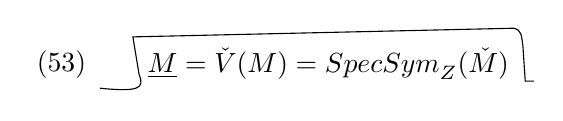
\begin{tikzpicture}[baseline=(eq.base)]
\node[anchor=base west,inner sep=0pt] (eq) at (0,0)
{$\underline{M}=\check{V}(M)=\operatorname{Spec}\operatorname{Sym}_{\mathbb{Z}}(\check{M})$};
\node[anchor=east] at ([xshift=-0.65cm]eq.west) {$(53)$};
\draw
([xshift=-0.60cm,yshift=-0.10cm]eq.south west)
.. controls ([xshift=-0.10cm,yshift=-0.15cm]eq.south west)
and ([xshift=-0.03cm,yshift=-0.10cm]eq.south west)
.. ([xshift=-0.10cm,yshift=0.07cm]eq.south west)
-- ([xshift=-0.18cm,yshift=0.14cm]eq.north west)
-- ([xshift=0.05cm,yshift=0.25cm]eq.north east)
.. controls ([xshift=0.16cm,yshift=0.23cm]eq.north east)
and ([xshift=0.15cm,yshift=0.15cm]eq.north east)
.. ([xshift=0.17cm,yshift=0.03cm]eq.north east)
-- ([xshift=0.20cm,yshift=-0.01cm]eq.south east)
-- ([xshift=0.31cm,yshift=-0.01cm]eq.south east);
\end{tikzpicture}}
denotes the vector bundle \unsure{covariant|canonical} in $M$ which it defines, and

\margin{27}

\scanpage{29}
\mspage{662}

where $M_0$ is one of the $M_i$, giving rise
to the system (cofinal in that of all the
$M_i$) of the $nM_0$. The choice of a
basis of $M_0$ over $\mathbb{Z}$ gives an
isomorphism
\[
(54)\qquad
\begin{aligned}
\operatorname{Env}^{0}(\mathcal{G})
&\simeq \operatorname{Env}^{0}(M_0)
\simeq \bigl(\operatorname{Env}^{0}(\mathbb{Z})^{\unsure{0}}\bigr)^n\\
&\simeq(\mathcal{E}^{1})^n
\end{aligned}
\]

\margin{$\unsure{\dagger}$ where
\diagram{\begin{tikzcd}[column sep=large]
(\mathbb{E}^{1},\unsure{mn|nm}) \arrow[r] &
(\mathbb{E}^{1},\uuline{n})
\end{tikzcd}}
is multiplication by $m$}

\[
(55)\qquad
\begin{aligned}
\mathcal{E}^{1}
&\simeq \operatorname{Env}^{0}(\mathbb{Z})
\simeq\operatorname{Spec}\bigl(\mathbb{Z}+T\mathbb{Q}[T]\bigr)\\
&\inserted{\simeq\varprojlim_n(\mathbb{E}^{1},n)\,\unsure{\dagger}}
\end{aligned}
\]
is the group scheme considered
above, which represents the group-valued functor
\[
(56)\qquad
A\longmapsto\mathcal{E}^{1}(A)
=\deleted{\unsure{\varprojlim}}
\left\{(x_n)\in A^{\mathbb{N}^{*}}\ \middle|\
\begin{gathered}
x_n=mx_{mn}\\[-2pt]
\forall m,n\in\unsure{\mathbb{N}^{*}}
\end{gathered}
\right\}.
\]

[If $A$ is such that there exists $n\in\mathbb{N}^{*}$ with
$nA\,\unsure{=|\simeq}\,0$ ---
\deleted{\unsure{precisely}}
which means
that the residue characteristics of $A$ divide $n$,
and \deleted{\unsure{it is}} there probably exists such an $n$
as soon as the residue characteristics of $A$ are
all $>0$ --- then $\mathcal{E}^{1}(A)=\{1\}$ ---
if on the other hand $A$ of characteristic $0$, we have $\mathcal{E}^{1}(A)\simeq A$]

\margin{28}

\scanpage{30}

5. \uline{Universal characterization} of the schematic envelope of a metabelian group.

Let $G$ be a group scheme \unsure{locally} of finite presentation over a base $S$.
We say that a \unsure{homomorphism} of group schemes
\diagram{\begin{tikzcd}
H \arrow[r] & G
\end{tikzcd}}
is \deleted{\unsure{quasi-}} \uline{unipotent} (resp. quasi-unipotent) if the image of $\forall$ \unsure{element} of $H$ is a unipotent element (resp. quasi unipotent) of $G$ --- which is checked fiber by fiber. A \unsure{homomorphism} from a discrete group
\diagram{\begin{tikzcd}
\mathcal{G} \arrow[r] & \Gamma(G/S)
\end{tikzcd}}
is said to be unipotent (resp. quasi-unipotent) if the \unsure{homomorphism} of group schemes \deleted{\unsure{associated}} \inserted{which} corresponds to it
\diagram{\begin{tikzcd}
\mathcal{G}_S \arrow[r] & G
\end{tikzcd}}
is unipotent (resp. quasi-unipotent).

\margin{29}

\scanpage{31}
\mspage{663}

Note that by the properties of $\varprojlim$ of filtered projective systems (with affine transition morphisms) \deleted{between} of schemes, if $\mathcal{G}$ is metabelian, whence a projective system of affine group schemes over $S_0$, hence over $S$, denoted $\operatorname{Env}_{\unsure{\underline{S}|S}}(\mathcal{G})$, and a projective limit
\[
\begin{aligned}
(57)\qquad L\operatorname{Env}_S(\mathcal{G})
 &=L\operatorname{Env}(\mathcal{G})\times_{S_0}S\\
 &\simeq\varprojlim\operatorname{Env}_S(\mathcal{G}),
\end{aligned}
\]
we have, as soon as $G$ is \unsure{locally} of finite presentation

\begin{samepage}
(58)\quad
\diagram{\begin{tikzcd}[column sep=large,row sep=large]
\operatorname{Hom}_{\mathrm{progr}/S}(\operatorname{Env}_S(\mathcal{G}),G)
 \arrow[r,"\sim"] \arrow[d,equal,"\mathrm{def}"']
 & \operatorname{Hom}(\operatorname{Env}_S(\mathcal{G}),G)\\
\varprojlim_i\unsure{\operatorname{Hom}}(\underline{\mathcal{G}}_{i\,S},G) &
\end{tikzcd}}
\end{samepage}

Note on the other hand that we have a \deleted{\unsure{a}} canonical \unsure{homomorphism}

\begin{samepage}
(59)\quad
\diagram{\begin{tikzcd}
\mathcal{G}_S \arrow[r] & \deleted{\unsure{\varprojlim}}L\operatorname{Env}_S(\mathcal{G})
\end{tikzcd}}
\end{samepage}
deduced by \unsure{change} of base from the \unsure{homomorphism} over the universal base $S_0$

\begin{samepage}
(59 bis)\quad
\diagram{\begin{tikzcd}
\mathcal{G}_{S_0} \arrow[r] & L\operatorname{Env}(\mathcal{G})
\end{tikzcd}}
\end{samepage}
coming from the system of canonical \unsure{homomorphisms}

\margin{30}

\scanpage{32}

\diagram{\begin{tikzcd}
\underline{\mathcal{G}}_{S_0}\arrow[r]&\underline{\mathcal{G}}_i
\end{tikzcd}}.

Thus, via (59) we find

\begin{samepage}
(60)\quad
\diagram{\begin{tikzcd}[column sep=large,row sep=large]
\operatorname{Hom}_{S\text{-}\mathrm{gr}}(L\operatorname{Env}_S(\mathcal{G}),G)
 \arrow[r] & \operatorname{Hom}_{S\text{-}\mathrm{gr}}(\mathcal{G}_S,G)
 \arrow[d,phantom,"\simeq"{rotate=90}]\\
 & \operatorname{Hom}_{\mathrm{gr}}(\mathcal{G},\Gamma(G/S))
\end{tikzcd}}
\end{samepage}

\unsure{1}

\unsure{Composing} (58) and (60), we find
\[
(61)\quad\left\{
\begin{aligned}
&\operatorname{Hom}_{\mathrm{pro}\text{-}S\text{-}\mathrm{gr}}\unsure{\ell}
 (\operatorname{Env}_S(\mathcal{G}),G)
 \simeq\operatorname{Hom}_{S\text{-}\mathrm{gr}}(L\operatorname{Env}_S(\mathcal{G}),G)\\[1.2em]
&\hspace{5em}\longrightarrow\operatorname{Hom}_{S\text{-}\mathrm{gr}}(\mathcal{G}_S,G)
 \simeq\operatorname{Hom}_{\mathrm{gr}}(\mathcal{G},G(S))
\end{aligned}\right.
\]
This being so, we have the following result

\Needspace{24\baselineskip}
\uline{Theorem} \deleted{\unsure{If}} Under the preceding conditions

\margin{\figure{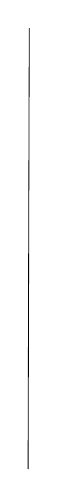
\begin{tikzpicture}
\draw[line width=.3pt] (0,0) -- (-.015,-5.6);
\end{tikzpicture}}}
($\mathcal{G}$ a discrete metabelian group, $G$ a group scheme locally of finite presentation over a base \unsure{scheme} $S$), the canonical map (61) is \deleted{\uline{bijective} if we assume moreover, so as not to tire \unsure{myself|oneself}, that} \inserted{injective, and has as image} \unsure{the set} of \unsure{homomorphisms} \uline{quasi-unipotent} from $\mathcal{G}$ into $G(S)$ --- at least if we assume, to simplify life for ourselves, that $S$ is \unsure{noetherian} and $G$ affine over $\unsure{S|S_0}$.

\margin{31}

\scanpage{33}
\mspage{664}

\uline{5\unsure{1|0}} \uline{Example} : The Fermat ``tower''.

1. The groups $\mathcal{G},\underline{\mathcal{G}}$.

I am interested in the quotient of $\mathcal{G}_0^{\deleted{\unsure{\wedge}}}=\operatorname{GL}(2,\mathbb{Z})$ obtained by taking the quotient by $[\Pi_0,\Pi_0]$ --- we find an extension $\mathcal{G}$ of $\mathcal{G}_0/\Pi_0$ by the group

\margin{$\Pi_0$ generated by the $\lambda_i=-\ell_i$,\quad
$\displaystyle \ell_0=\begin{pmatrix}1&-2\\0&1\end{pmatrix}$\quad
$\displaystyle \ell_1=\begin{pmatrix}1&0\\2&1\end{pmatrix}$.}

\[
\begin{aligned}
(1)\qquad M\overset{\mathrm{dfn}}{=}\Pi_{0\,\mathrm{ab}}
\simeq
\Bigl(
\underset{\deleted{\underbrace{\hphantom{\mathbb{Z}(0)+\mathbb{Z}(1)+\mathbb{Z}(\infty)}}_{M}}}
{\overset{\deleted{\unsure{\wedge}}}{\mathbb{Z}}(0)+
 \overset{\deleted{\unsure{\wedge}}}{\mathbb{Z}}(1)+
 \overset{\deleted{\unsure{\wedge}}}{\mathbb{Z}}(\infty)}
\Bigr)/\text{diagonal}
\end{aligned}
\]
Thus we have an exact sequence of profinite groups

\begin{samepage}
(2)\quad
\diagram{\begin{tikzcd}[column sep=large,row sep=large]
1\arrow[r] & M\arrow[r]\arrow[d,phantom,"\simeq"{rotate=90}]
 &\mathcal{G}\arrow[r]
 &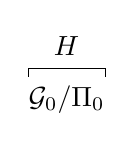
\begin{tikzpicture}[baseline=(q33.base)]
\node[inner sep=0pt] (q33) {$\mathcal{G}_0/\Pi_0$};
\draw[line width=.3pt] ([yshift=3pt]q33.north west)--([yshift=6pt]q33.north west)--([yshift=6pt]q33.north east)--([yshift=3pt]q33.north east);
\node[above=7pt] at (q33.north) {$H$};
\end{tikzpicture}\arrow[r]\arrow[d,phantom,"\simeq"{rotate=90}]
 &1\\
 &\begin{gathered}\Pi_{0\,\mathrm{ab}},\text{ also denoted}\\\mathcal{G}^{\circ}\end{gathered}
 &&\operatorname{GL}(2,\mathbb{Z}/4\mathbb{Z})/(\dot{\ell}_0,\dot{\ell}_1)&
\end{tikzcd}}
\end{samepage}

In terms of generators and relations we have
\[
(3)\quad\mathcal{G}=\left\{\tau',\rho,\sigma\;\middle|\;
\begin{aligned}
&\rho^6=\sigma^4={\tau'}^2=1\\
&\rho^3=\sigma^2,\quad\tau'(\rho)=\rho^{-1},\quad\tau'(\sigma)=\sigma^{-1}\\
&\deleted{\unsure{\rho}}[\lambda_0,\lambda_1]=1,\quad\text{where}
\end{aligned}\right.
\]
\[
\hspace{8em}\left\{
\begin{aligned}
\lambda_0&=-\ell_0=-\sigma\rho\sigma\rho=\sigma(\rho)\rho^{\deleted{\unsure{-1|4}}}\\
\lambda_1&=-\ell_1=-\rho\sigma\rho\sigma=\rho\sigma(\rho)
\end{aligned}\right.
\]
\unsure{of which|thus} the commutation relation $[\lambda_0,\lambda_1]=1$ is also written
\[
(4)\qquad \sigma(\rho)\rho^2\sigma(\rho)=\rho\sigma(\rho^2)\rho
\qquad\text{or again}
\]
\[
(5)\qquad -\sigma\underbrace{\rho\sigma\rho^{-1}\sigma\rho}\sigma
=\underbrace{\rho\sigma\rho^{-1}\sigma\rho}
\]
where the play of the $-$ signs can be made explicit in the formalism of generators and relations by removing this sign from the formula, and replacing in \unsure{return} one (or an odd \unsure{num\textsuperscript{b}er|number}) of the $\sigma$ in the formula by $\sigma^{-1}$. For example, the formula

\margin{32}

\scanpage{34}

is written, introducing

\margin{\uline{N.B.} $\lambda_\infty\overset{\mathrm{dfn}}{=}-\ell_\infty$}

\[
(6)\qquad
\lambda_\infty\deleted{\unsure{=-\ell_\infty}}
=\rho\sigma\rho^{-1}\sigma\rho
=\rho(\sigma)\sigma\rho
=-\rho\sigma(\rho)^{-1}\rho
=\rho\sigma\rho^{-1}(\sigma)
\]
in the form
\[
(7)\qquad [\sigma,\lambda_\infty]=1.
\]
\margin{N.B. $\sigma=\sigma_\infty$}

\margin{\uline{N.B.} We find
\[
\left\{
\begin{aligned}
[\ell_0,\ell_1]&=[\lambda_0,\lambda_1]=(\sigma(\rho)\rho^{-1})^3\\
[\underbrace{\sigma_{\deleted{\unsure{\infty}}}}_{\sigma}\unsure{,}\ell_\infty]
&=[\underbrace{\sigma_\infty}_{\sigma},\lambda_\infty]
=(\sigma(\rho^{-1})\rho)^3\\
&=\operatorname{int}(\sigma\rho^{-1})\cdot[\ell_0,\ell_1]
\end{aligned}\right.
\]}

We are going to define a group scheme \inserted{$\underline{\mathcal{G}}$} over $\mathbb{Z}$, whose \inserted{$\unsure{\widehat{\mathbb{Z}}|\mathbb{Z}}$-}points will be \inserted{(up to an \unsure{isomorphism} say)} the points of $\widehat{\mathcal{G}}$. We put
\[
(8)\qquad
\underline{M}=\underline{\mathcal{G}}^{\circ}
=\unsure{\mathbb{G}_a|\mathbb{E}_a}^{\{0,1,\infty\}}/\text{diagonal}
\]
\margin{It is better to \unsure{denote} it by $\underline{M}$ --- there are already too many $\mathcal{G}$'s!}

We are going to have \deleted{$\unsure{\mathcal{G}/M}$}
\[
\deleted{(\unsure{4})}(4)\qquad
\mathcal{G}\deleted{\unsure{=\operatorname{GL}(2,\mathbb{Z})}}
\simeq\operatorname{GL}(2,\mathbb{Z})/[\Pi_0,\Pi_0]
\]
operate on $\underline{M}\deleted{\unsure{=\underline{\mathcal{G}}^{\circ}}}$,
\deleted{\unsure{by describing in this way}} \inserted{through}
\[
(5)\qquad
\underbrace{\mathcal{G}_3\times\mu_{\unsure{\tau|2}}^{\deleted{\unsure{2}}}}_{\simeq\unsure{T_{0,3}|\Gamma_{0,3}}}
\simeq\mathcal{G}/M\deleted{\unsure{\widehat{\mathbb{Z}}}}
\simeq\mathcal{G}_{0,3}/\Pi.
\]

Denoting by $\unsure{\overbrace{\dot{\lambda}_0,\dot{\lambda}_1}},\dot{\lambda}_\infty$ the images of the
$\deleted{\lambda_0,\lambda_1}\lambda_i=-\ell_i$ in $\deleted{\unsure{M}}\mathcal{G}$, identified with elements of
\[
M=\mathcal{G}^{\circ}=\underline{\mathcal{G}}^{\circ}(\widehat{\mathbb{Z}})
\]
--- in fact we have
\[
(6)\qquad
\left\{
\begin{aligned}
\dot{\lambda}_0\unsure{,|>}\dot{\lambda}_1,\dot{\lambda}_\infty
&\in\deleted{\unsure{\underline{\mathcal{G}}^{\circ}}}\inserted{\underline{M}}(\mathbb{Z})
\subset\deleted{\unsure{\underline{\mathcal{G}}^{\circ}}}\inserted{\underline{M}}(\widehat{\mathbb{Z}})
=M\otimes_{\unsure{\cdot|\mathbb{Z}}}\unsure{\mathbb{Z}|\widehat{\mathbb{Z}}}\\
\text{thus,}\quad\dot{\lambda}_0+\dot{\lambda}_1+\dot{\lambda}_\infty&=0
\end{aligned}\right.
\]
\margin{(here we write the group law in $M=\underline{\mathcal{G}}^{\circ}$ additively)}

\margin{\figure{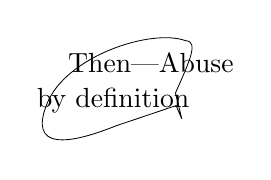
\begin{tikzpicture}[scale=.8]
\draw[line width=.3pt] (1.2,.85) .. controls (.65,1.05) and (-.7,.6) .. (-1,-.15)
 .. controls (-1.3,-.9) and (-.65,-.8) .. (.1,-.5)
 -- (1.05,-.18) -- (1.14,-.39) -- (1.04,.02)
 .. controls (1.25,.5) and (1.42,.84) .. (1.2,.85);
\node at (.65,.5) {\unsure{Then|Abuse}};
\node at (.05,-.1) {by definition};
\end{tikzpicture}}}
$\mathcal{G}_3$ operates on $\underline{M}=\underline{\mathcal{G}}^{\circ}$ by its action on the canonical \deleted{\unsure{bases}} \inserted{generators} $\deleted{\unsure{\lambda_0}}\dot{\lambda}_0,\dot{\lambda}_1,\dot{\lambda}_\infty$, thus
\[
(7)\qquad
\left\{
\begin{aligned}
\sigma(\dot{\lambda}_0)&=\dot{\lambda}_1,\quad
\sigma(\dot{\lambda}_1)=\dot{\lambda}_0
\quad\inserted{\text{hence}}\quad
\sigma(\dot{\lambda}_\infty)=\dot{\lambda}_\infty\\
\rho(\dot{\lambda}_i)&=\dot{\lambda}_{i+1}
\end{aligned}\right.
\]
\margin{This is seen first for $i=0,1$ and, \unsure{is deduced from it} for $i=\infty$.}
On the other hand we have by definition
\[
(8)\qquad\tau(\dot{\lambda}_i)=-\dot{\lambda}_i
\]
where
\diagram{\begin{tikzcd}[column sep=2pt,row sep=small]
\tau\arrow[d,equal]&{}={}&\sigma&\tau'\arrow[d,equal]\\
\tau_\infty&&&\tau'_\infty
\end{tikzcd}}

\margin{33}

\scanpage{35}
\mspage{665}

. The announced extension $\underline{\mathcal G}$ is of course that of § 50 3°), \unsure{developed} in the meantime (since the first lines of the present §, noting precisely that I was feeling cramped in making the construction explicit) :

\begin{samepage}
(9)\quad\diagram{\begin{tikzcd}[column sep=large]
1 \arrow[r] & \underline M \arrow[r] \arrow[d,equal] & \underline{\mathcal G} \arrow[r] & H_{S_0} \arrow[r,no head] & 1 \\
 & \check V(M) & & &
\end{tikzcd}}
\end{samepage}
where $S_0=\operatorname{Spec}\mathbb Z$.

For $\unsure{\forall}$ scheme $S$, we will put
\[
\tag{10}
\begin{gathered}
\underline{\mathcal G}^{\Delta}(S)\subset\underline{\mathcal G}(S)\\
\Vert\;\mathrm{dfn}\\
\text{Inverse image of the ``diagonal'' of}\\
\Gamma(H_{\unsure{S|S_0}}/S)
\quad\bigl(\text{i.e. of the image of }H\longrightarrow\Gamma(H_{\unsure{S|S_0}},S)\bigr)\\
\text{under the canonical homomorphism }\underline{\unsure{\mathcal G|\mathcal E}}(S)\longrightarrow H_S(S),
\end{gathered}
\]
so that by the construction of loc. cit. we will have a canonical isomorphism
\[
\tag{11}
\underline{\mathcal G}^{\Delta}(S)\simeq
\mathcal G\underset{M}{\wedge}\deleted{\unsure{A}}
\underbrace{\Gamma(S,\underline{\mathcal O}_S\otimes_{\mathbb Z}M)}_{
\simeq\deleted{\unsure{A}}\inserted{M}\otimes_{\mathbb Z}A\ \text{if}}
\]
and a canonical exact sequence

\begin{samepage}
(12)\quad\diagram{\begin{tikzcd}[column sep=large]
1 \arrow[r] & \underbrace{\Gamma(S,\underline{\mathcal O}_S\otimes_{\mathbb Z}M)}_{A\otimes_{\mathbb Z}M} \arrow[r] & \underline{\mathcal G}^{\Delta}(S) \arrow[r] & H \arrow[r] & 1.
\end{tikzcd}}
\end{samepage}

\figure{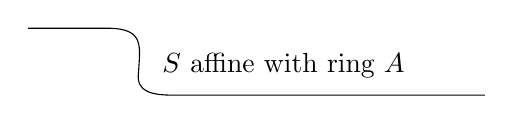
\begin{tikzpicture}[x=1cm,y=1cm]
\draw (0,0.75) -- (1.0,0.75)
.. controls (1.48,0.75) and (1.42,0.53) .. (1.40,0.18)
.. controls (1.37,-0.06) and (1.57,-0.10) .. (1.85,-0.10)
-- (5.80,-0.10);
\node[anchor=west] at (1.58,0.28) {$S$ affine with ring $A$};
\end{tikzpicture}}

Taking $A=\widehat{\mathbb Z}$, we find in particular (and this is again a general fact about group schemes associated with extensions of discrete groups with abelian kernel)
\[
\tag{13}
\mathcal G^{\wedge}\simeq\underline{\mathcal G}^{\Delta}(\widehat{\mathbb Z}).
\]
\margin{34}

\scanpage{36}

2. The group $\widetilde Z_{\rho,\sigma}$ : \uline{provisional version}.

. I am now going to make explicit for $\widehat{\mathcal G}$ and $\widehat{\mathcal G}_{\unsure{0|\bullet}}\longrightarrow\widehat{\mathcal G}$ the general constructions of § 49 $\overline{\underline{\mathrm{VI}}}$, taking \inserted{there} \deleted{$\unsure{\mathcal G}$}
\[
\tag{14}
\underline{\mathcal G}^{\unsure{\natural}}\overset{\mathrm{dfn}}=
\underline M=\underline{\mathcal G}^{\circ}
\quad(\text{identity component of }\underline{\mathcal G})
\]
In a case like this one, where $\underline{\mathcal G}^{\unsure{\natural}}$ is precisely the closed subgroup of the $(\rho,\sigma)$-group $\mathcal G_{\rho,\sigma}$ $(=\mathcal G^{\wedge}\text{ here})$ generated by $\lambda_0,\lambda_1,\lambda_\infty$, we \unsure{will dispense} in the notation --- where there is no ambiguity --- with including the notation $\unsure{\natural}$. For \unsure{$\forall$ $A$} we will have to distinguish for example between $G_{\rho,\sigma}$ and $G_{\rho,\sigma}^{\unsure{\natural}}$ etc. \uline{We will however carry out the constructions in the scheme-theoretic setting, rather than the profinite one.}

\margin{I think I will compare the two possible constructions at the end. The \unsure{underlines} will indicate the group \uline{schemes}...}

The essential step is to determine the group $\underline Z_{\rho,\sigma}$
\[
\tag{15}
\begin{gathered}
\underline Z_{\rho,\sigma}\subset\underline{\operatorname{Aut}}(\underline{\mathcal G}^{+})\\
\Vert\;\mathrm{dfn}\\
\left\{u\in\underline{\operatorname{Aut}}(\mathcal G^{+})\ \left|\
\begin{aligned}
\deleted{\unsure{1^{\circ}}}\ \text{a)}\;&\exists\alpha\in\underline{\mathcal G}_{\tau}^{\unsure{\natural}}=\{1,\tau\}.\underline M,
&&u(\rho)=\alpha(\rho)\\
\text{b)}\;&\exists\beta\in\text{-- -- -- -- -- --}
&&u(\sigma)=\beta(\sigma)\\
\text{c)}\;&u(L_0^{\deleted{\unsure{\Pi_0}}\mathcal G})=L_0^{\mathcal G}
&&\deleted{\unsure{(\Longleftrightarrow L_0^{\Pi_0}=L_0^{\natural})}}\\
&\qquad(\Longleftrightarrow u(L_0^{\Pi_0})=L_0^{\Pi_0})\\
\bigl[\text{d)}\;&(\text{automatic})\quad u(\mathcal G^{\unsure{\natural}})\subset\mathcal G^{\unsure{\natural}}\bigr]
\end{aligned}\right.\right.
\end{gathered}
\]

\margin{here, ``$\exists\alpha$'' ``$\exists\beta$'' of course means the \uline{local} existence of $\alpha,\beta$...}

Let us note that $u$ is determined by the values
\[
\tag{16}
\begin{cases}
u(\rho)=\xi\rho\\
u(\sigma)=\eta\sigma
\end{cases}
\qquad\xi,\eta\in\Gamma\underline\Pi
\]
\margin{where $\underline\Pi=\underline M\unsure{\rtimes}\deleted{\unsure{\{1,\tau\}}}\inserted{\unsure{\mu_2}}$ ($\underline M$ \unsure{subgroup|is a group} of index $2$ in $\underline\Pi$)}
\inserted{$\xi,\eta$} satisfying the following conditions ;
\margin{35}

\scanpage{37}
\mspage{666}

\[
\tag{17}
\left\{
\begin{aligned}
\text{a)}\;&\xi\rho\ \text{(locally) conjugate to }\rho\ \text{via }\underline{\unsure{\mathcal G}}^{\unsure{\natural}}=\underline M\\
\text{b)}\;&\eta\sigma\ \text{-- -- -- -- -- -- ---}\ \sigma\ \text{'' -- -- ---}\\
\text{c)}\;&\text{loop equation}\\
&\xi=\eta\ell_1^{\nu}\quad\text{where }\nu\in\Gamma\mathbb G_a\ \text{suitable}\\
&\qquad\bigl(\text{such that }\mu\overset{\mathrm{dfn}}=2\nu+1\in\Gamma\mathbb G_m\bigr)
\end{aligned}\right.
\]

. \deleted{Since $\xi,\eta\in\Gamma N$, it will be necessary}

\uline{Remark} It is no longer possible here to denote by $-1$ the nontrivial element \inserted{$\omega$} of the center $\unsure{\mu|\mu_2}$ of $\mathcal G^{\wedge}$, and to denote by $-x$ (for $x\in\mathcal G^{\wedge}$) the product of $x$ with it, because of the confusion with the notation $-x$ \inserted{(for $x\in M$)} in the abelian group $M$ for the inverse of $x$ --- but \deleted{\unsure{the element}} $\omega x\ne-x$, since $\omega x\notin M$, $-x\in M$...

We of course put
\[
\tag{18}
\varepsilon_3(u)=\varepsilon_{\mathcal G}(\alpha),\qquad
\varepsilon_2(u)=\varepsilon_{\mathcal G}(\beta)
\]
(well defined, since $\rho$ and $\rho^{-1}$ are not conjugate on any fiber, idem for $\sigma,\sigma^{-1}$), how to make them explicit in terms of $\xi,\eta$ ? We will have

\deleted{\unsure{(17)}}
\[
\tag{19}
\left\{
\begin{aligned}
\xi=\alpha\rho(\alpha)^{-1}
&\left\{
\begin{aligned}
&\in\Gamma\underline M\quad\text{if }\alpha\in\Gamma\underline M=\Gamma\underline{\mathcal G}^{\unsure{\natural}}\ \text{i.e. }\varepsilon_3(u)=1\\
&=\underbrace{\alpha_0}_{\in\Gamma\underline M}\tau\rho(\alpha_0\tau)^{-1}
=\alpha_0\underbrace{(-\ell_1^{-1})}_{\lambda_1^{-1}\in\underline M}\rho(\alpha_0)^{-1}\in\Gamma\underline M\quad\text{if }\varepsilon_3(u)=\unsure{-1}
\end{aligned}\right.\\[1ex]
\eta=\beta\sigma(\beta)^{-1}
&\left\{
\begin{aligned}
&\in\Gamma\underline M\quad\text{if }\beta\in\Gamma\underline M=\Gamma\underline{\mathcal G}^{\unsure{\natural}}\ \text{i.e. }\varepsilon_2(u)=1\\
&=(\underbrace{\beta_0}_{\in\Gamma\underline M}\tau)\sigma(\beta_0\tau)^{-1}
=\omega\beta_0\sigma(\beta_0)^{-1}\in\omega\underline M\quad\text{if }\varepsilon_2(u)=\unsure{-1}
\end{aligned}\right.
\end{aligned}\right.
\]
thus in any case
\[
\tag{19 bis}
\begin{cases}
\xi\in\Gamma\underline M\\
\eta\in\Gamma\bigl(\omega^{\nu_2(u)}.\underline{M}\bigr)
\end{cases}
\]
\margin{36}

\scanpage{38}
\mspage{676}

from which we get, by the loop equation (17)
\[
\tag{20}
\ell_1^{\nu}=(\omega\lambda_1)^{\nu}\in\Gamma(\omega^{\nu_2(u)}.\underline M)
\quad\text{i.e. }\unsure{\Longleftrightarrow}\ \omega^{\nu}\in\Gamma(\omega^{\nu_2(u)}.\underline M)
\]
We can write it in the form
\[
\tag{21}
\underline\nu=2\underline\nu'+\underline\nu_2
\]
where
\[
\tag{22}
\left\{
\begin{aligned}
\underline\nu,\underline\nu' &: Z_{\rho,\sigma}\longrightarrow\mathbb G_a\\
\underline\nu_2,\underline\nu_3 &: Z_{\rho,\sigma}\rightrightarrows
(\mathbb Z/2\mathbb Z)_{S_0}^{\unsure{\mathrm{que}|\mathrm{cste}}}
\end{aligned}\right.
\]
\deleted{$\unsure{\varepsilon}$}
are well-defined \unsure{morphisms} of schemes, related \inserted{to one another and} to the group homomorphisms \deleted{$\unsure{\mu}$}
\[
\underline\mu:Z_{\rho,\sigma}\longrightarrow\mathbb G_m,\qquad
\underline\varepsilon_{\unsure{1|2}},\underline\varepsilon_3:Z_{\rho,\sigma}\longrightarrow\{\pm1\}_{S_0}
\]
by the formulas (21) and
\[
\tag{23}
\left\{
\begin{aligned}
\underline\mu&=2\underline\nu\,\unsure{+}\,1\deleted{\unsure{+1}}
\quad(=4\underline\nu'\,\unsure{+}\,2\underline\nu_2+1)\\
\underline\varepsilon_2&=(-1)^{\underline\nu_2},\qquad
\underline\varepsilon_3=(-1)^{\underline\nu_3}.
\end{aligned}\right.
\]

We will therefore have, by virtue of (\unsure{24|21})
\deleted{
\[
\tag{24}
\ell_1^{\nu}=\ell_1^{2\nu'}\ell_1^{\nu_2}
=\underbrace{(\omega\lambda_1)}_{\lambda_1}^{2\nu'}\ell_1^{\nu_2}
=\lambda_1^{2\nu'}\ell_1^{\nu_2}
\]
Since $\ell_1=\lambda_1\omega$, we
\deleted{I feel like putting the $\ell_i$ in the form}
\[
\tag{25}
\ell_i=a_i\omega\quad\text{where }a_i\in\underline M!
\]
can \deleted{\unsure{to thus|will be able to}} write (24) in the form
\[
\tag{26}
\ell_1^{\nu}=\underbrace{(\lambda_1^{\unsure{2\nu'}}a_1^{\nu_2})}_{\in\Gamma\underline M}\omega^{\nu_2}
\quad\deleted{\text{for }\unsure{\nu_2=0|\nu_2=1}\ \text{i.e. }\unsure{\varepsilon_2=1}}
\]
To make the $a_i$ explicit, we must expand them as linear combinations of $\lambda_0,\lambda_1,\lambda_\infty$ (or of two of them, if we want uniqueness).
}
\margin{37}
